\subsubsection*{Training Insights}


As mentioned in \cref{train_params}, I decided to not use 4000 epochs of training for the basic network. To explain why, consider \autoref{fig:basic_cnn_overf}. This plot shows the training history for the basic model and the previously mentioned training parameters. The validation loss has a minimum after just 90 epochs of training and keeps on rising until reaching a steady level for the rest of the training. The training loss though keeps on decreasing for the whole training. This indicates that the model reached a certain amount of accuracy quickly but as training progressed, it started to overfit the individual images and accuracy on the validation set decreased. 

\begin{figure}[H]
\centering
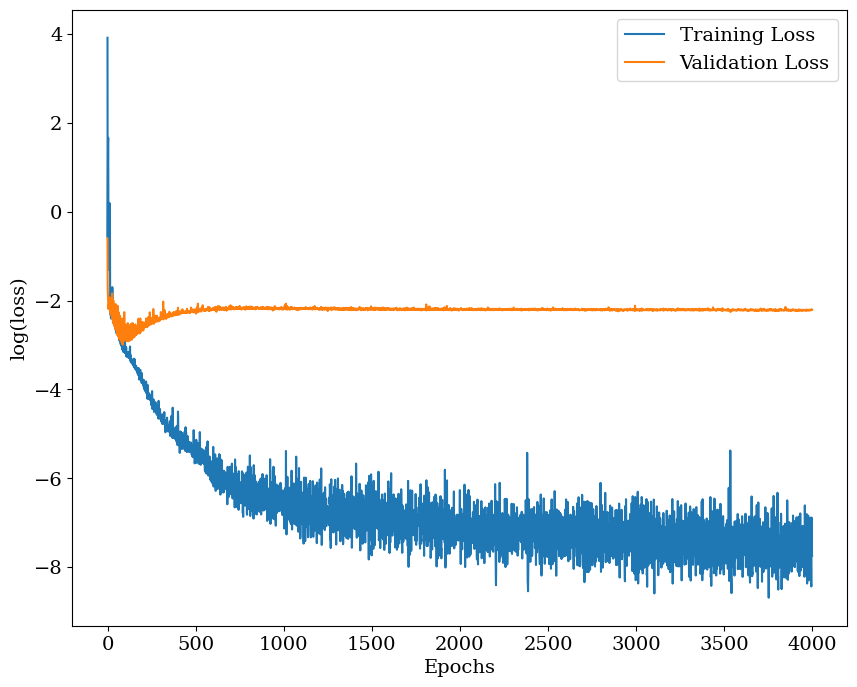
\includegraphics[width=.667\textwidth]{images/Chapter4/Basic CNN/hist_overf.png}
\caption{Training history for the basic CNN model. While the training loss is continuously getting lower, the validation loss reached its minimum after around 100 epochs, indicating overfitting. The validation loss reached a value of 0.130 and the training loss of 0.0006 after 4000 epochs of training.} 
\label{fig:basic_cnn_overf}
\end{figure}

We would expect the predictions on the test set to be way worse than the predictions on the training set. To examine this, consider \autoref{fig:overf_comp} and \ref{fig:overf_comp_hist}.

\begin{figure}[H]
\centering
\begin{subfigure}{.46\textwidth}
  \centering
  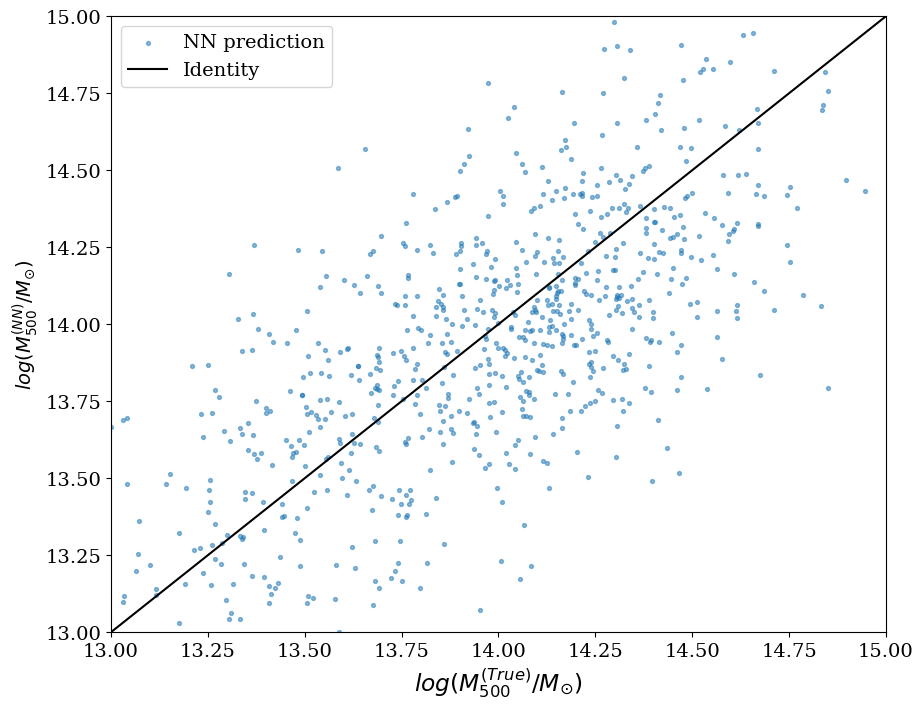
\includegraphics[width=\linewidth]{images/Chapter4/Basic CNN/overf_test_set.png}
  \caption{Model predictions on the test set.}
  \label{fig:overf_comp_test}
\end{subfigure}%
\hspace{.6em}
\begin{subfigure}{.46\textwidth}
  \centering
  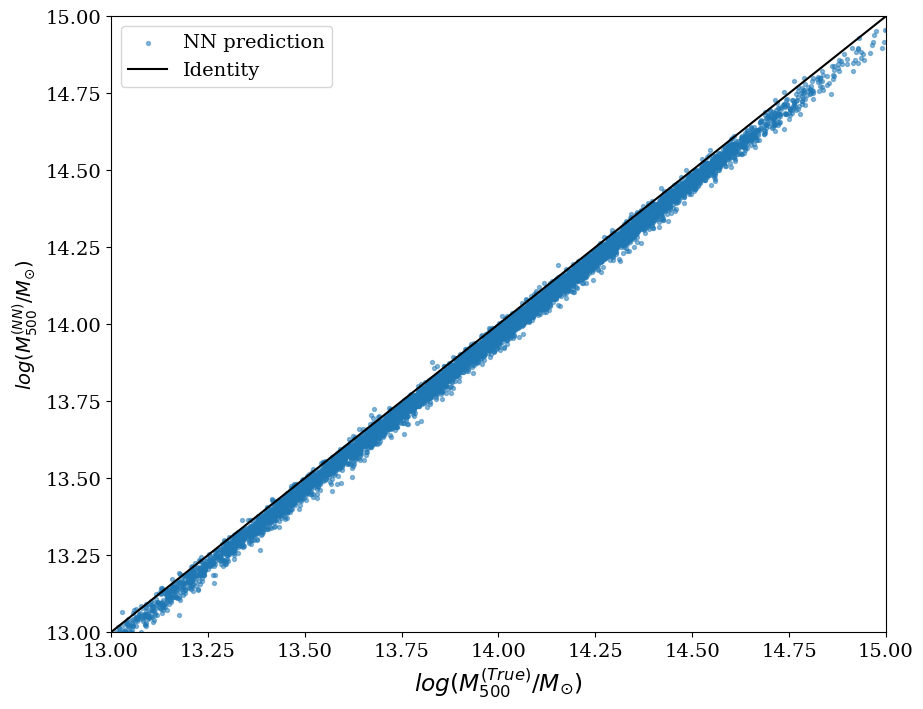
\includegraphics[width=\linewidth]{images/Chapter4/Basic CNN/overf_test_trainset.png}
  \caption{Model predictions on the training set.}
  \label{fig:overf_comp_train}
\end{subfigure}
\caption{Difference between the test and the training predictions of the trained model. The x-axis shows the true mass and the y-axis the predicted mass. The very exact predictions on the training set indicate overfitting which is confirmed by the bad predictions on the test set.} 
\label{fig:overf_comp}
\end{figure}

\begin{figure}[H]
\centering
\begin{subfigure}{.46\textwidth}
  \centering
  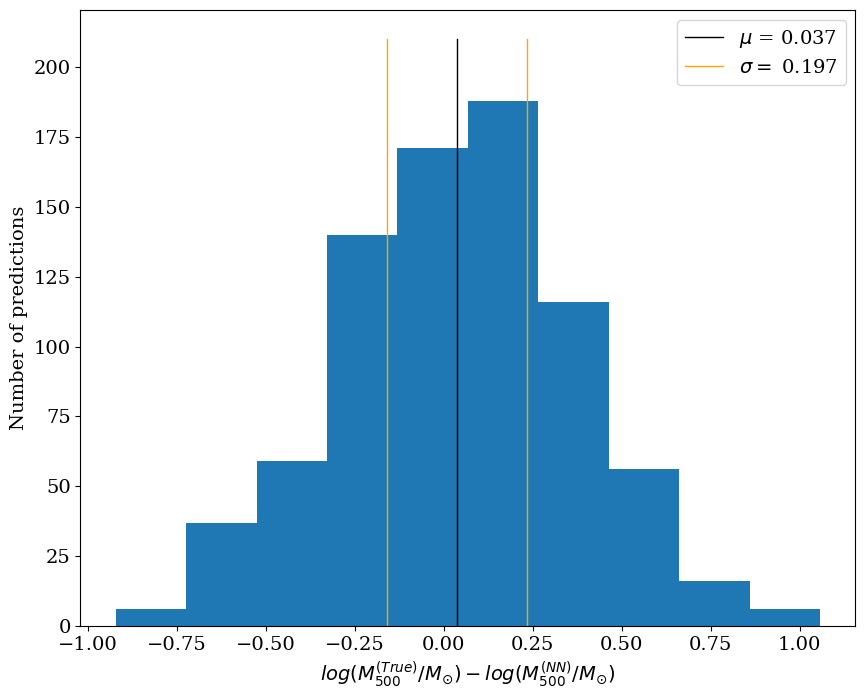
\includegraphics[width=\linewidth]{images/Chapter4/Basic CNN/overf_test_set_hist.png}
  \caption{Histogram of model predictions on the test set.}
  \label{fig:overf_comp_test_hist}
\end{subfigure}%
\hspace{.6em}
\begin{subfigure}{.46\textwidth}
  \centering
  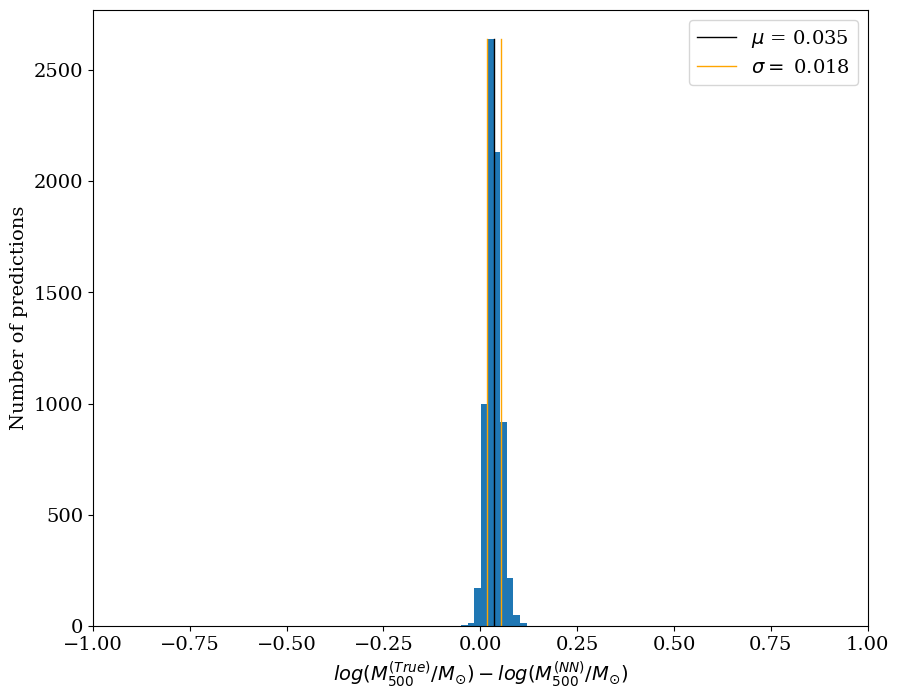
\includegraphics[width=\linewidth]{images/Chapter4/Basic CNN/overf_train_set_hist.png}
  \caption{Histogram of model predictions on the training set.}
  \label{fig:overf_comp_train_hist}
\end{subfigure}
\caption{Looking at the difference between the actual mass an the predicted mass, it is easy to spot the overfitting. It also indicates that the model is predicting somewhat smaller than the actual masses.} 
\label{fig:overf_comp_hist}
\end{figure}

Knowing what overfitting looks like now, we can try to improve our training. There are countless ways to do that. One could stop the training earlier, for example at around 100 epochs where the validation loss was at a minimum. Another way would be to lower the learning rate. This allows the model to train more slowly and maybe find another solution to more accurate predictions that do not encourage overfitting. 

\begin{figure}[H]
\centering
\begin{subfigure}{.46\textwidth}
\centering
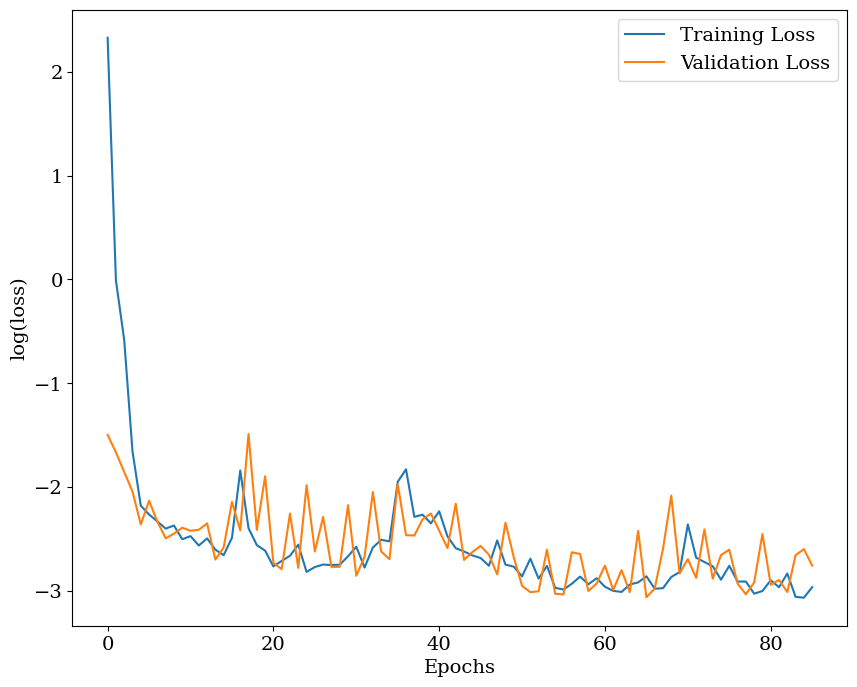
\includegraphics[width=\textwidth]{images/Chapter4/Basic CNN/best_perf_historie.png}
\caption{Training history for the best basic CNN model with a learning rate of 0.001, stopped after around 90 epochs.} 
\label{fig:comp_learning_rates_a}
\end{subfigure}
\hspace{.6em}
\begin{subfigure}{.46\textwidth}
\centering
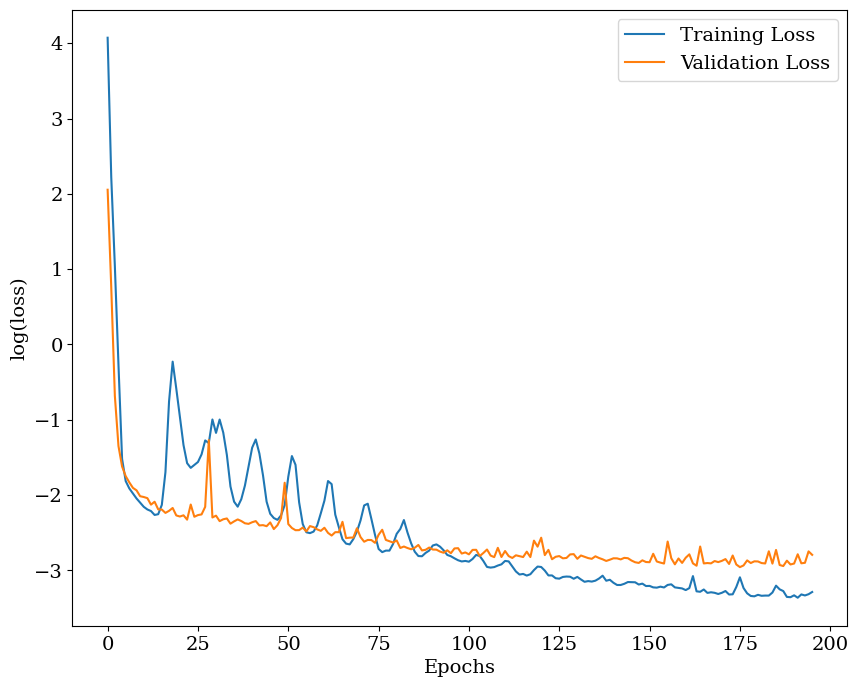
\includegraphics[width=\textwidth]{images/Chapter4/Basic CNN/hist_learning_rate.png}
\caption{Training history for the basic CNN model with a learning rate of 0.0005, stopped after around 190 epochs.} 
\label{fig:comp_learning_rates_b}
\end{subfigure}
\caption{A learning rate of $0.001$ (\textit{left}) compared to a learning rate of $0.0005$ (\textit{right}). The training with a lower learning rate reached its validation loss minimum after around double the epochs of the training with the standard learning rate of $0.001$.}
\label{fig:comp_learning_rates}
\end{figure}

There were no huge differences between these two approaches to prevent overfitting. The two shown trainings (\autoref{fig:comp_learning_rates}) produced similar results, with the standard learning rate (\autoref{fig:comp_learning_rates_a}) being a bit more accurate which could be due to training randomness. In more trainings, the slower learning rate could sometimes beat the standard learning rate. I decided to keep the standard learning rate and use a feature called \textit{early stopping} for the basic CNN. It keeps track of the validation loss and stops training as soon as it does not improve for a given amount of epochs. It is then possible to save the model with the lowest validation loss.

Let's take a look at what the predictions look like for stopping the training earlier:

\begin{figure}[H]
\centering
\begin{subfigure}{.46\textwidth}
  \centering
  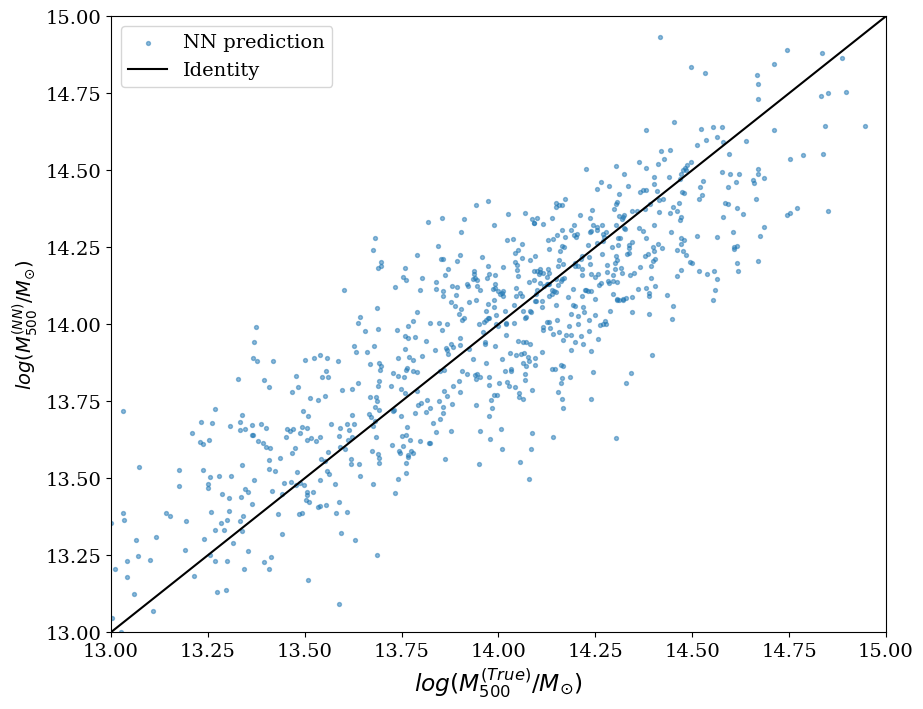
\includegraphics[width=\linewidth]{images/Chapter4/Basic CNN/best_perf_test.png}
  \caption{Model predictions on the test set.}
\end{subfigure}%
\hspace{.6em}
\begin{subfigure}{.46\textwidth}
  \centering
  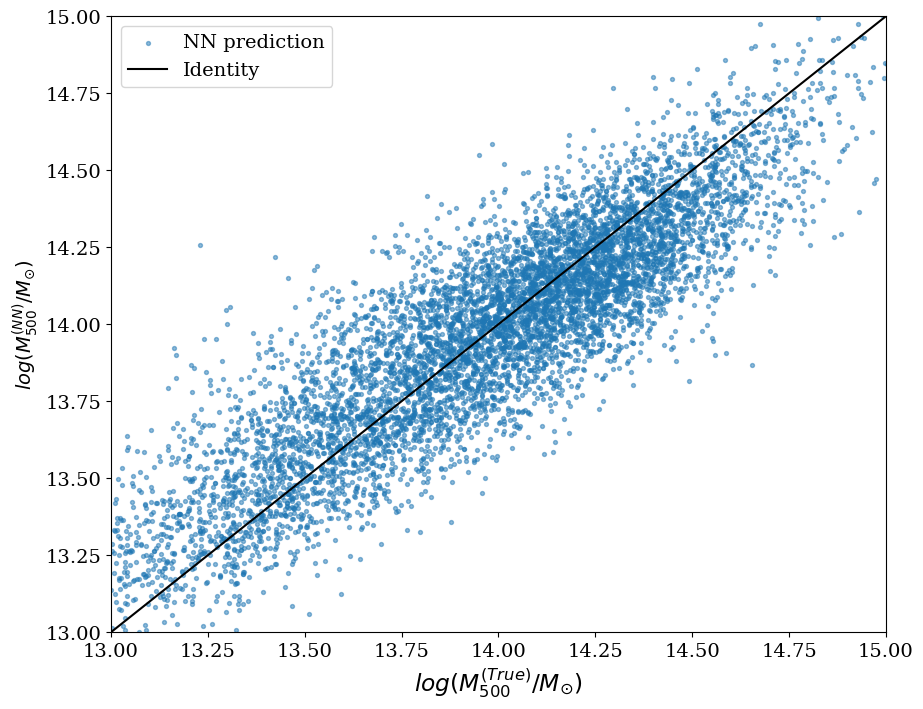
\includegraphics[width=\linewidth]{images/Chapter4/Basic CNN/best_perf_train.png}
  \caption{Model predictions on the training set.}
\end{subfigure}
\caption{Difference between the test and the training predictions of the trained model from \autoref{fig:comp_learning_rates_a}. This time the predictions on the test set are better than before (see \autoref{fig:overf_comp}) while the predictions on the training set are worse which indicates no, or only little overfitting.} 
\label{fig:short_training_comp}
\end{figure}

\begin{figure}[H]
\centering
\begin{subfigure}{.46\textwidth}
  \centering
  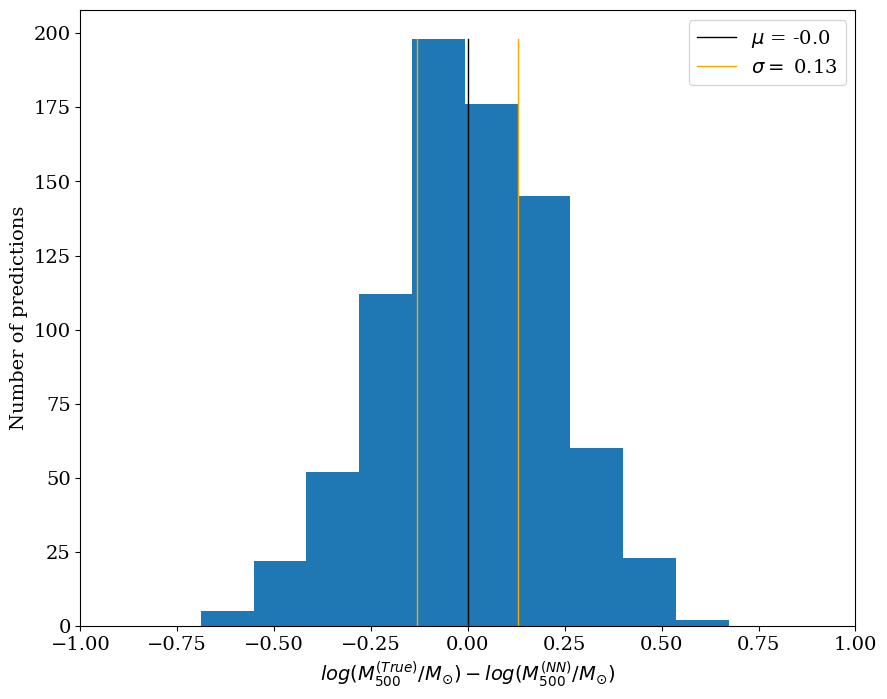
\includegraphics[width=\linewidth]{images/Chapter4/Basic CNN/best_perf_test_hist.png}
  \caption{Histogram of model predictions on the test set.}
\end{subfigure}%
\hspace{.6em}
\begin{subfigure}{.46\textwidth}
  \centering
  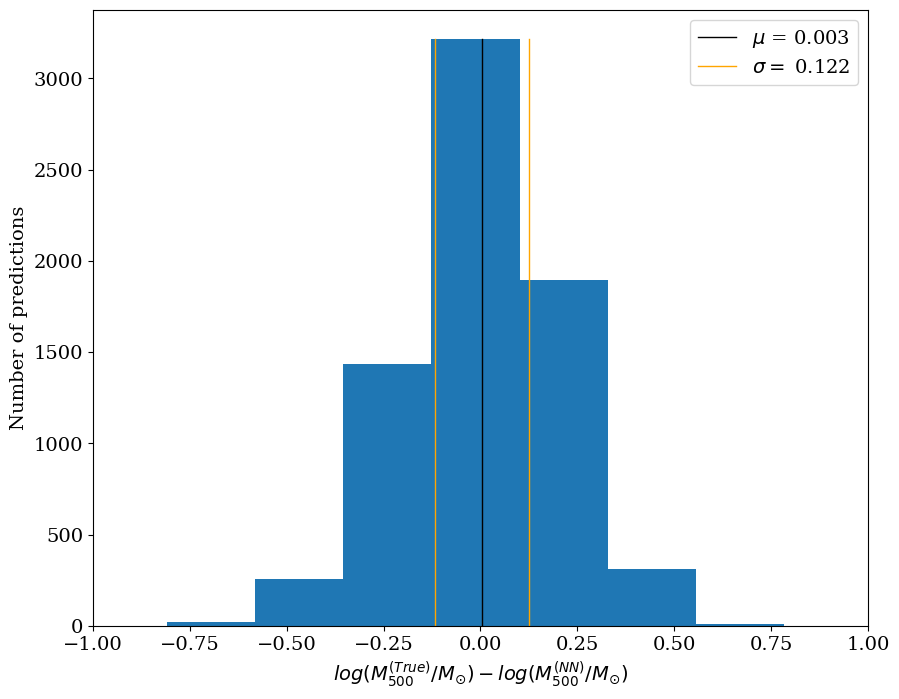
\includegraphics[width=\linewidth]{images/Chapter4/Basic CNN/best_perf_train_hist.png}
  \caption{Histogram of model predictions on the training set.}
\end{subfigure}
\caption{Now the histograms look way more similar to each other, which is exactly what we are looking for. This is also confirmed by the lower standard deviation of the difference between the actual and the predicted mass compared to the overfitted model.} 
\label{fig:short_training_comp_hist}
\end{figure}

For the basic CNN and for the deep models, I made a run of ten trainings each and will discuss their performance in the following sections starting with the best performing basic CNN.

\subsubsection*{Best Performing Model}

The best performing basic CNN reached its validation loss minimum after around 90 epochs of training. Compared to other trainings, it seemed to have picked up a useful filter early on as both the training and validation loss decrease significantly after only a few epochs. The predictions are nicely spread around the identity (see \autoref{fig:short_training_comp}) and consequently the average $\mu$ of the difference between the true and the predicted value is almost zero.\\
It is worth noting that this is already an improved model with an improved number of epochs to avoid overfitting. Moreover, the model's parameters were chosen to work for the given task by \citet{Krippendorf_2023}. For the deep models, the amount of epochs is set to 4000 and no other optimizations is done. \\

Normally, one would try to avoid overfitting where possible. In our case though, it is fine if we will observe overfitting, because we want to investigate whether a model is able to predict galaxy cluster masses in any way. If a model is not even able to make decent predictions on the training set after a few thousand epochs of training, it won't be suitable for our goal while a model that overfits massively after the training is at least able to find features within the images and is worth taking a deeper look at and optimizing later on. Because of that I will solely focus on the training results after 4000 epochs of training without any optimization.
